\section*{CHAPTER 1. INTRODUCTION}
\addcontentsline{toc}{section}{\numberline{}CHAPTER 1. INTRODUCTION}
\setcounter{section}{1}
\setcounter{subsection}{0}
\setcounter{figure}{0}
\setcounter{table}{0}

In a single carrier communication system, the symbol period must be much 
greater than the delay time in order to avoid inter-symbol interference (ISI) \cite{b1}. Since 
data rate is inversely proportional to symbol period, having long symbol periods 
means low data rate and communication inefficiency. A multicarrier system, such as 
FDM (aka: Frequency Division Multiplexing), divides the total available bandwidth 
in the spectrum into sub-bands for multiple carriers to transmit in parallel \cite{b2}. An 
overall high data rate can be achieved by placing carriers closely in the spectrum. 
However, inter-carrier interference (ICI) will occur due to lack of spacing to separate 
the carriers. To avoid inter-carrier interference, guard bands will need to be placed in 
between any adjacent carriers, which results in lowered data rate. 

OFDM (aka: Orthogonal Frequency Division Multiplexing) is a multicarrier 
digital communication scheme to solve both issues. It combines a large number of 
low data rate carriers to construct a composite high data rate communication system. 
Orthogonality gives the carriers a valid reason to be closely spaced, even overlapped, 
without inter-carrier interference. Low data rate of each carrier implies long symbol 
periods, which greatly diminishes inter-symbol interference \cite{b3}. 

Although the idea of OFDM started back in 1966 \cite{b4}, it has never been widely 
utilized until the last decade when it “becomes the modem of choice in wireless 
applications” \cite{b5}. It is now interested enough to experiment some insides of OFDM. 

The objective of this project is to demonstrate the concept and feasibility of an 
OFDM system, and investigate how its performance is changed by varying some of 
its major parameters. This objective is met by developing a MATLAB program to 
simulate a basic OFDM system. From the process of this development, the 
mechanism of an OFDM system can be studied; and with a completed MATLAB 
program, the characteristics of an OFDM system can be explored. 

\subsection{How to use latex}

\subsubsection{Table making}

    \begin{table}[H]
        \centering
        \caption{Experiment results}
        \begin{tabularx}{0.85\textwidth}{
            | >{\centering}y%\arraybackslash}y
            | >{\centering\arraybackslash}a
            | >{\centering\arraybackslash}a
            | >{\centering\arraybackslash}y|
            }
                \hline
            \bfseries  No.   &\bfseries Voltage \hspace{1cm}(mV)   &\bfseries Reference \hspace{0pt} (mV)  & \bfseries Error \hspace{0pt}(\%)\\\hline
             1  &   &   &\\\hline
             2  &   &   &\\\hline
             3  &   &   &\\\hline
        ...  &   &   &\\\hline
        \end{tabularx}
            \label{bang31}
    \end{table}

\subsubsection{Equation}
    \begin{equation}\label{pt31}
        F(x) = \int^a_b \frac{1}{3}x^3
    \end{equation}
    
Equation \ref{pt31} is an example of an integral equation.

\subsubsection{Add figure}
\begin{figure}[h]
    \centering
    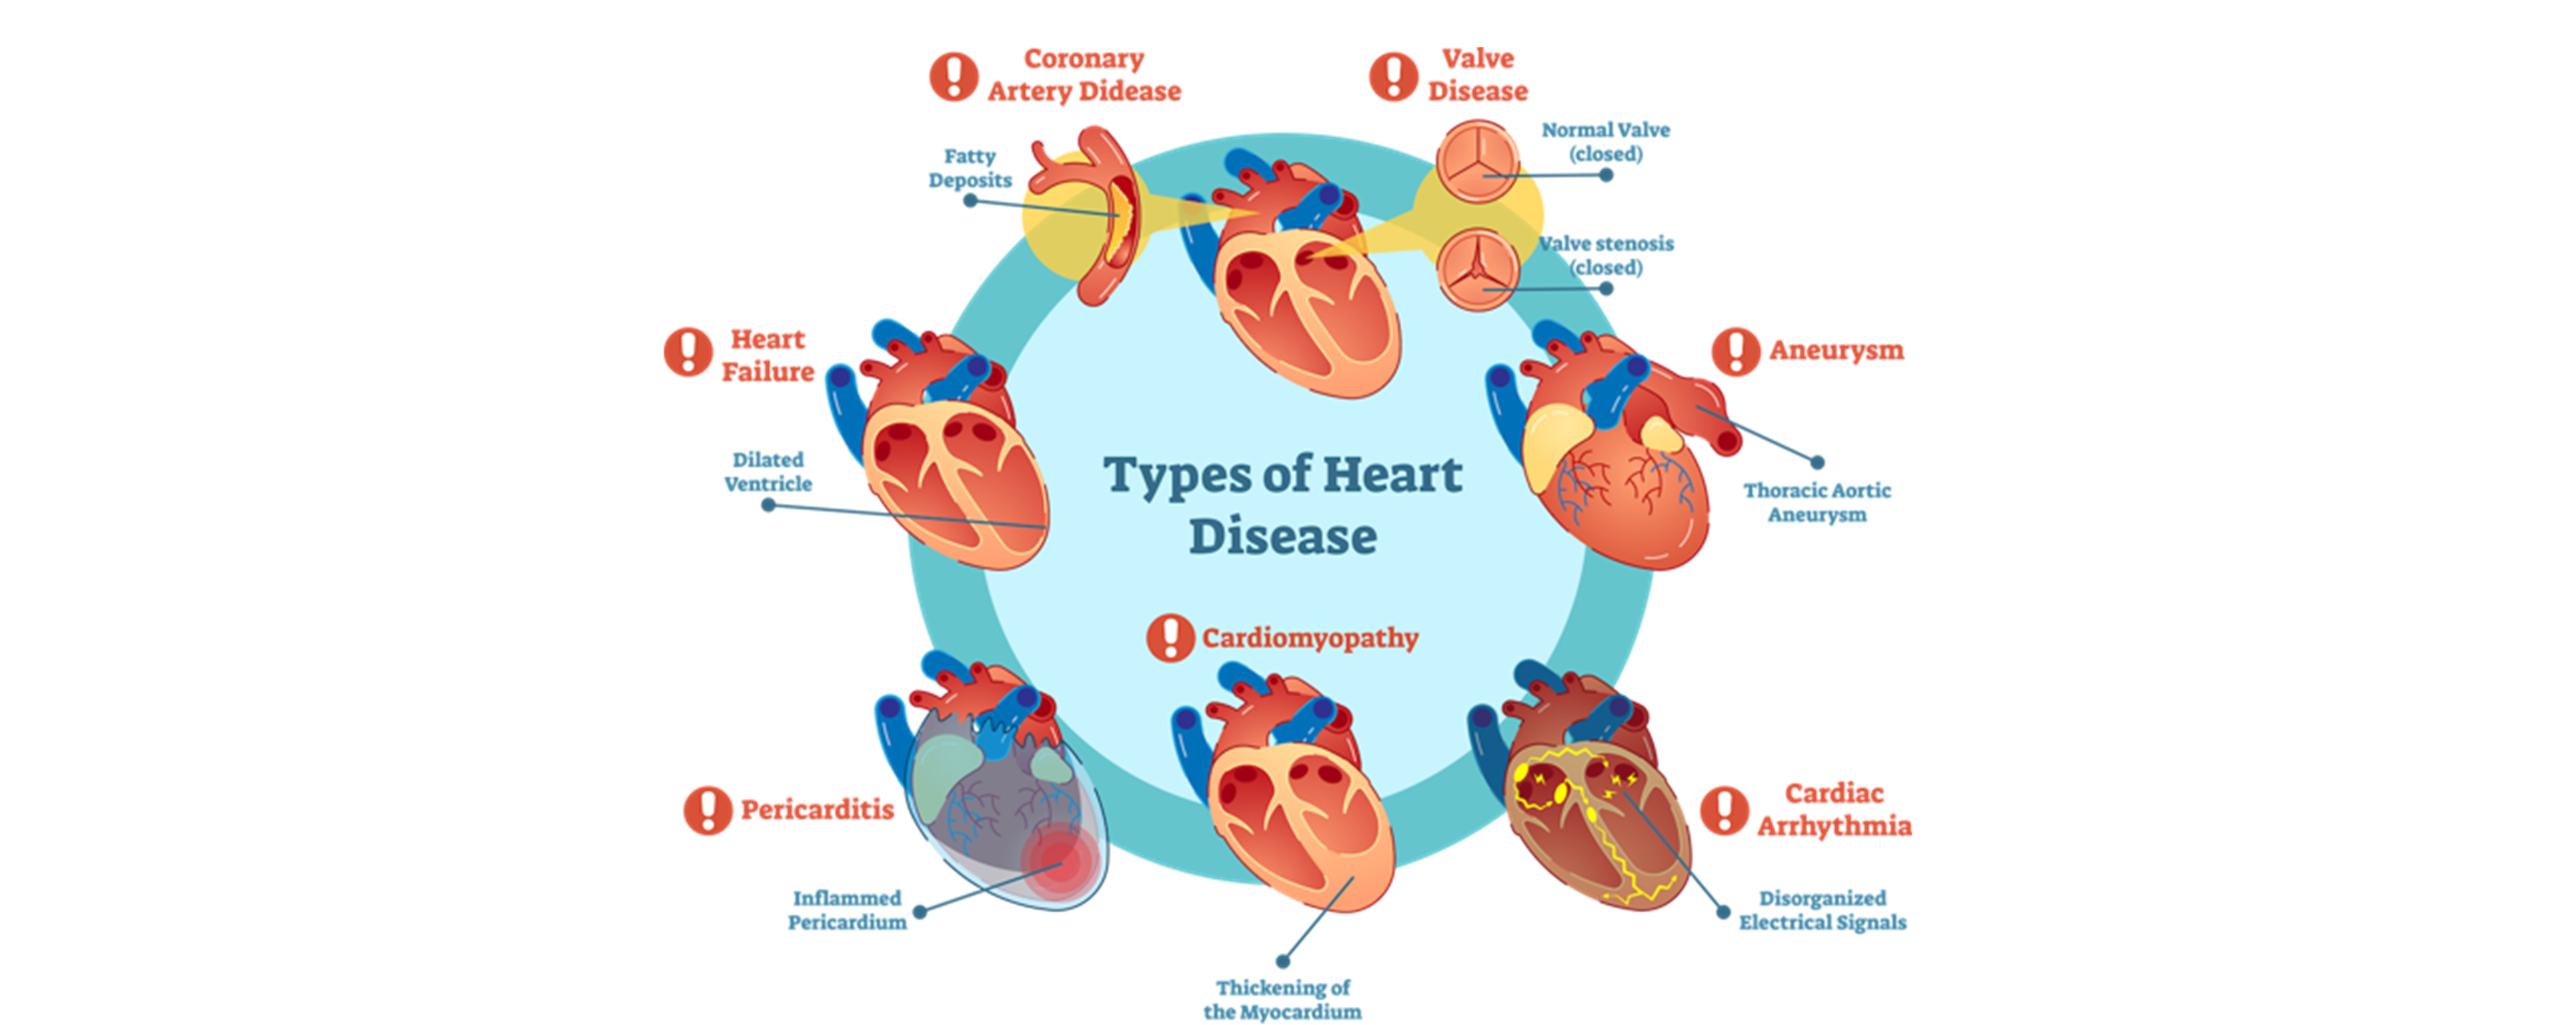
\includegraphics[width=1\textwidth]{Figures/Fig0.png}
    \caption{\bfseries\centering\fontsize{13pt}{0pt}\selectfont Heart disease}
    \label{fig1}
\end{figure}

Figure \ref{fig1} shows some heart disease \cite{b1}.